\section{System Overview}\label{overview}

Figure~\ref{fig:monolithic} presents an architectural overview of a
modern operating system with a monolithic kernel and Figure~\ref{fig:base IDDR system overview} 
presents the architectural overview of the IDDR system.

\begin{figure}[!ht]
\centering
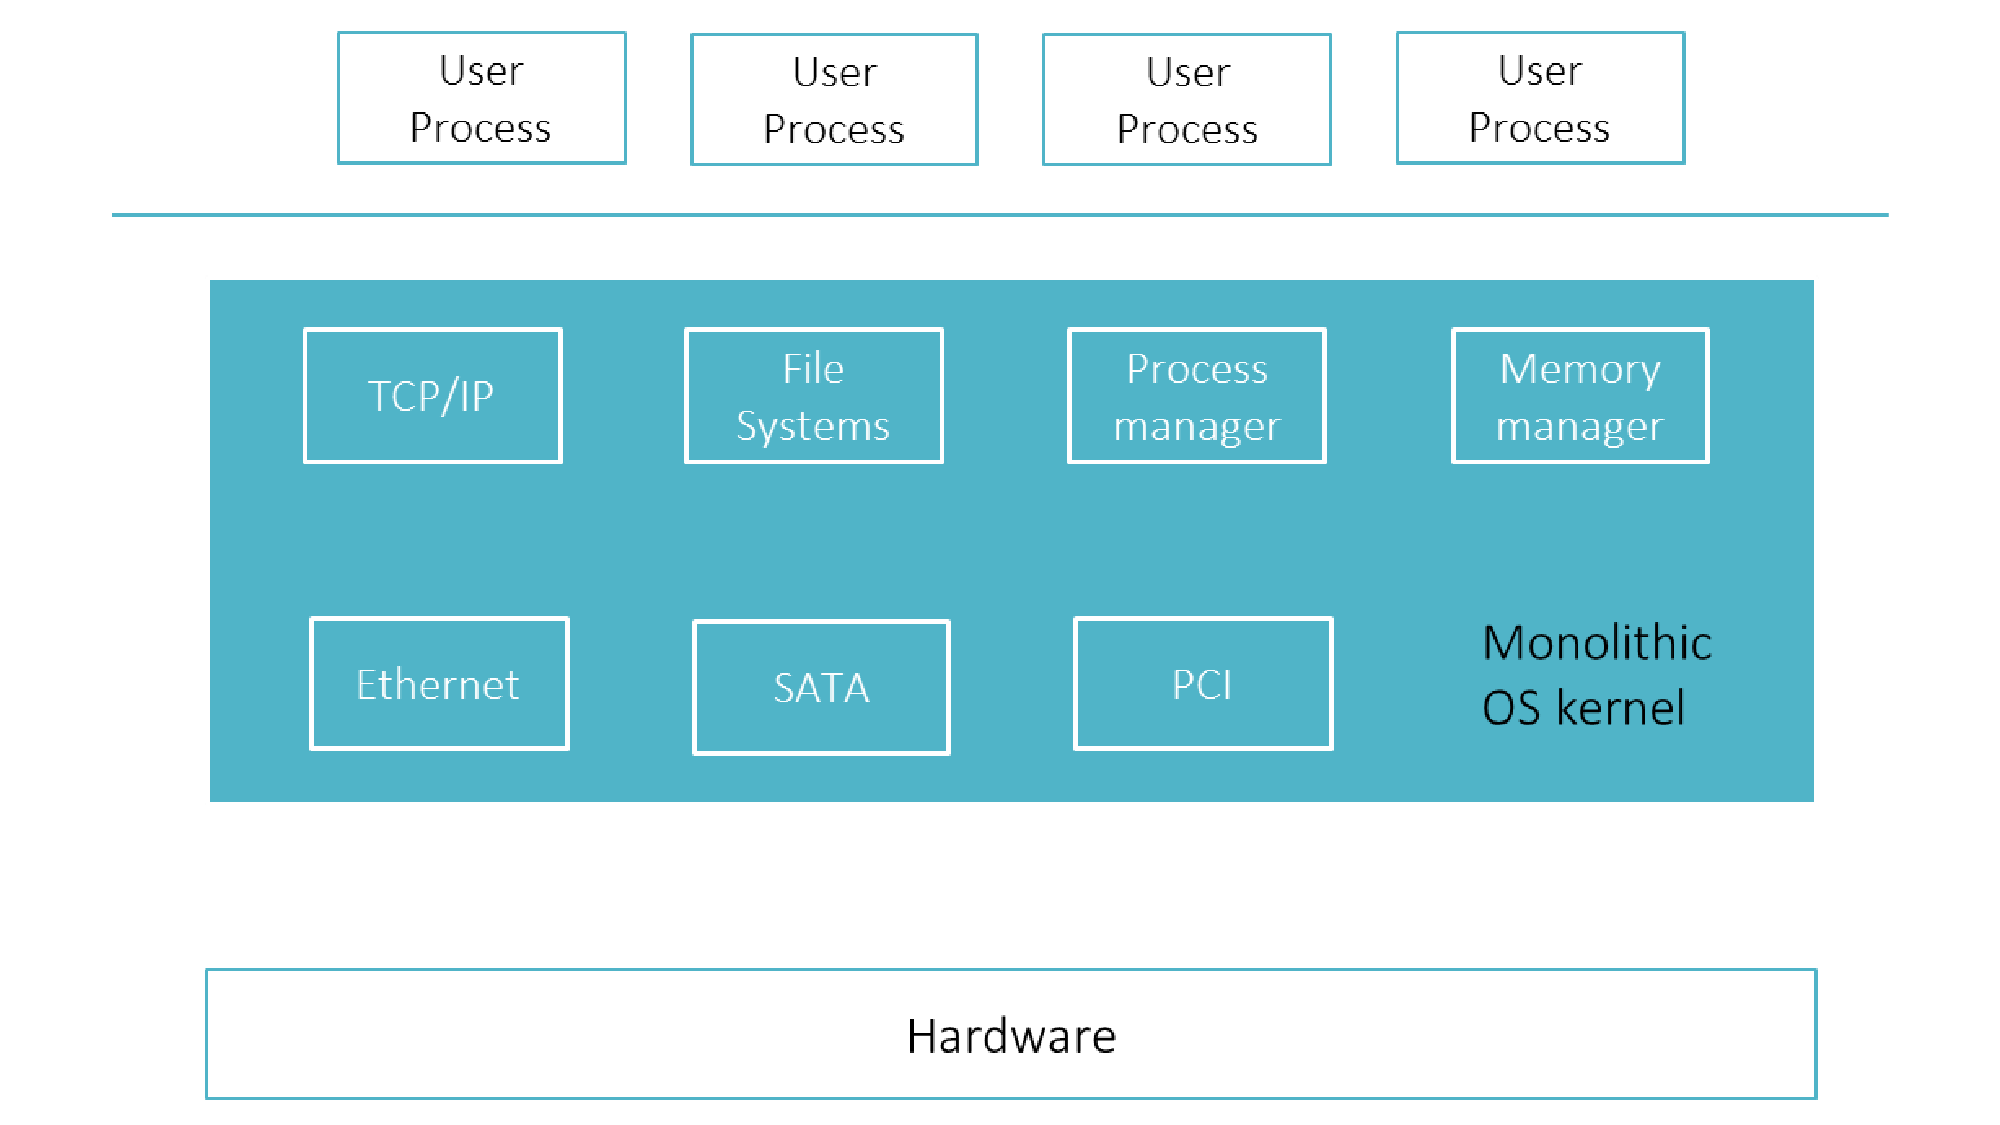
\includegraphics[scale=.5]{OSoverview}
\caption{Architectural overview of a modern OS}
\label{fig:monolithic}
\end{figure}

\begin{figure}[!ht]
\centering
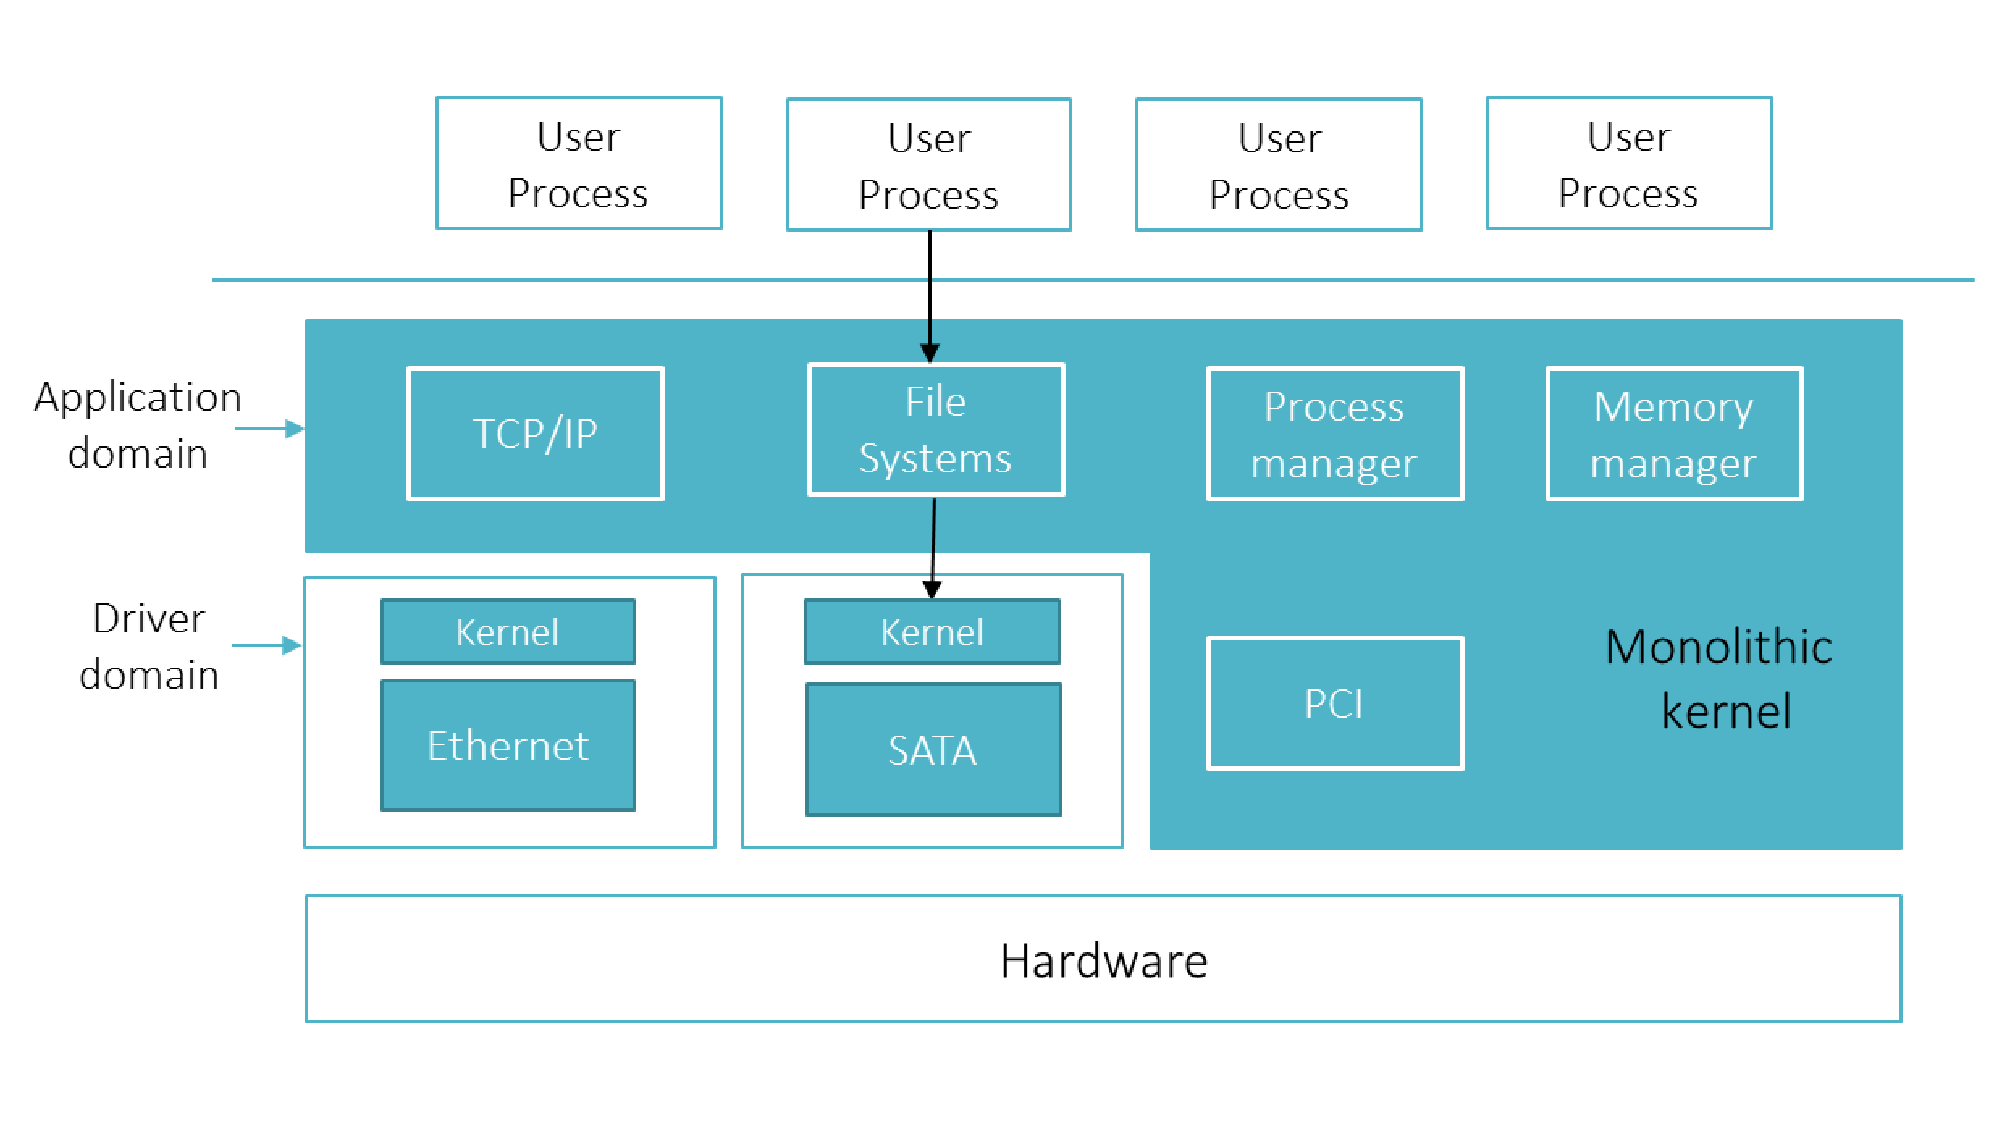
\includegraphics[scale=.5]{baseIDDRsystemoverview}
\caption{Architectural overview of the interrupt based IDDR system}
\label{fig:base IDDR system overview}
\end{figure}

Figure~\ref{fig:base IDDR system overview} shows that the IDDR
system partitions an existing kernel into multiple independent
components.  User applications and the Linux kernel run in a domain
called the \textit{application domain}. A device driver, which needs
to be isolated from a kernel, executes in the separate domain called
the \textit{driver domain}. Multiple domains run on the same hardware
with the help of a VMM. User applications or kernel components access
the hardware through the driver domain.

\section{Design Goals}\label{sec:goals}
The goal of isolated driver domains is to provide strong isolation
between a device driver and a monolithic kernel and at the same time to
avoid modifications to the device driver code. The goal of this thesis
is to reduce the performance penalty due to the required communication 
between domains when using this approach.

\subsection*{Sources of Overhead}
\label{subsec:overhead}
The IDDR system is a re-implementation of isolated driver domains proposed
by Fraser et. al. Even though the IDDR system provides better robustness
for the operating system, it suffers from performance overheads. The
main reasons for the lower performance are the data copying overhead
and the interdomain communication overhead.

\paragraph{Copying Overhead: } For write operations, the Linux kernel copies
data from user space to kernel space and then from kernel space to the
physical device. However, when using isolated driver domains, the system copies data
first from the guest OS's user space to guest OS's kernel space, then
to a shared memory segment, and from there to the physical
device. This extra copy lowers the performance of the system.

\paragraph{Communication Channel Overhead: } The application domain and
the driver domain send virtual interrupts when requests and responses
are shared between both domains. These virtual interrupts cause
a resumption of the receiving domain in order to deliver the them.  Resuming
a domain causes a context switch at the hypervisor level, which adds
overhead. Our goal is to reduce this context switch-related overhead by
reducing the frequency of context switches.

\section{Design Properties}
\label{sec:properties}
This section covers the properties of isolated driver domains, which our
performance optimizations must not compromise.

\subsection*{Strong Isolation}
Isolated driver domains provide strong fault isolation between the 
kernel and the device drivers. This isolation ensures that a bug within 
a device driver does not affect other kernel components.

\subsection*{Compatibility and Transparency} 
Alternative approaches to isolation, such as microkernels, require
changes to the kernel API that is presented to applications and drivers.
Consequently, existing applications and drivers will require substantial
changes to work under those designs.
By contrast, isolated driver domains do not change APIs visible to
applications and device driver code and hence existing device drivers
and applications are compatible with the new architecture.
Moreover, since the frontend drivers in the application domain
provides a standard device driver interface, its use is transparent
to the filesystem layer using them.


\section{System Components}\label{components}

This section describes the 3 main components of our design 
- the frontend driver, backend driver, and communication module.

\begin{figure}[!ht]
\centering
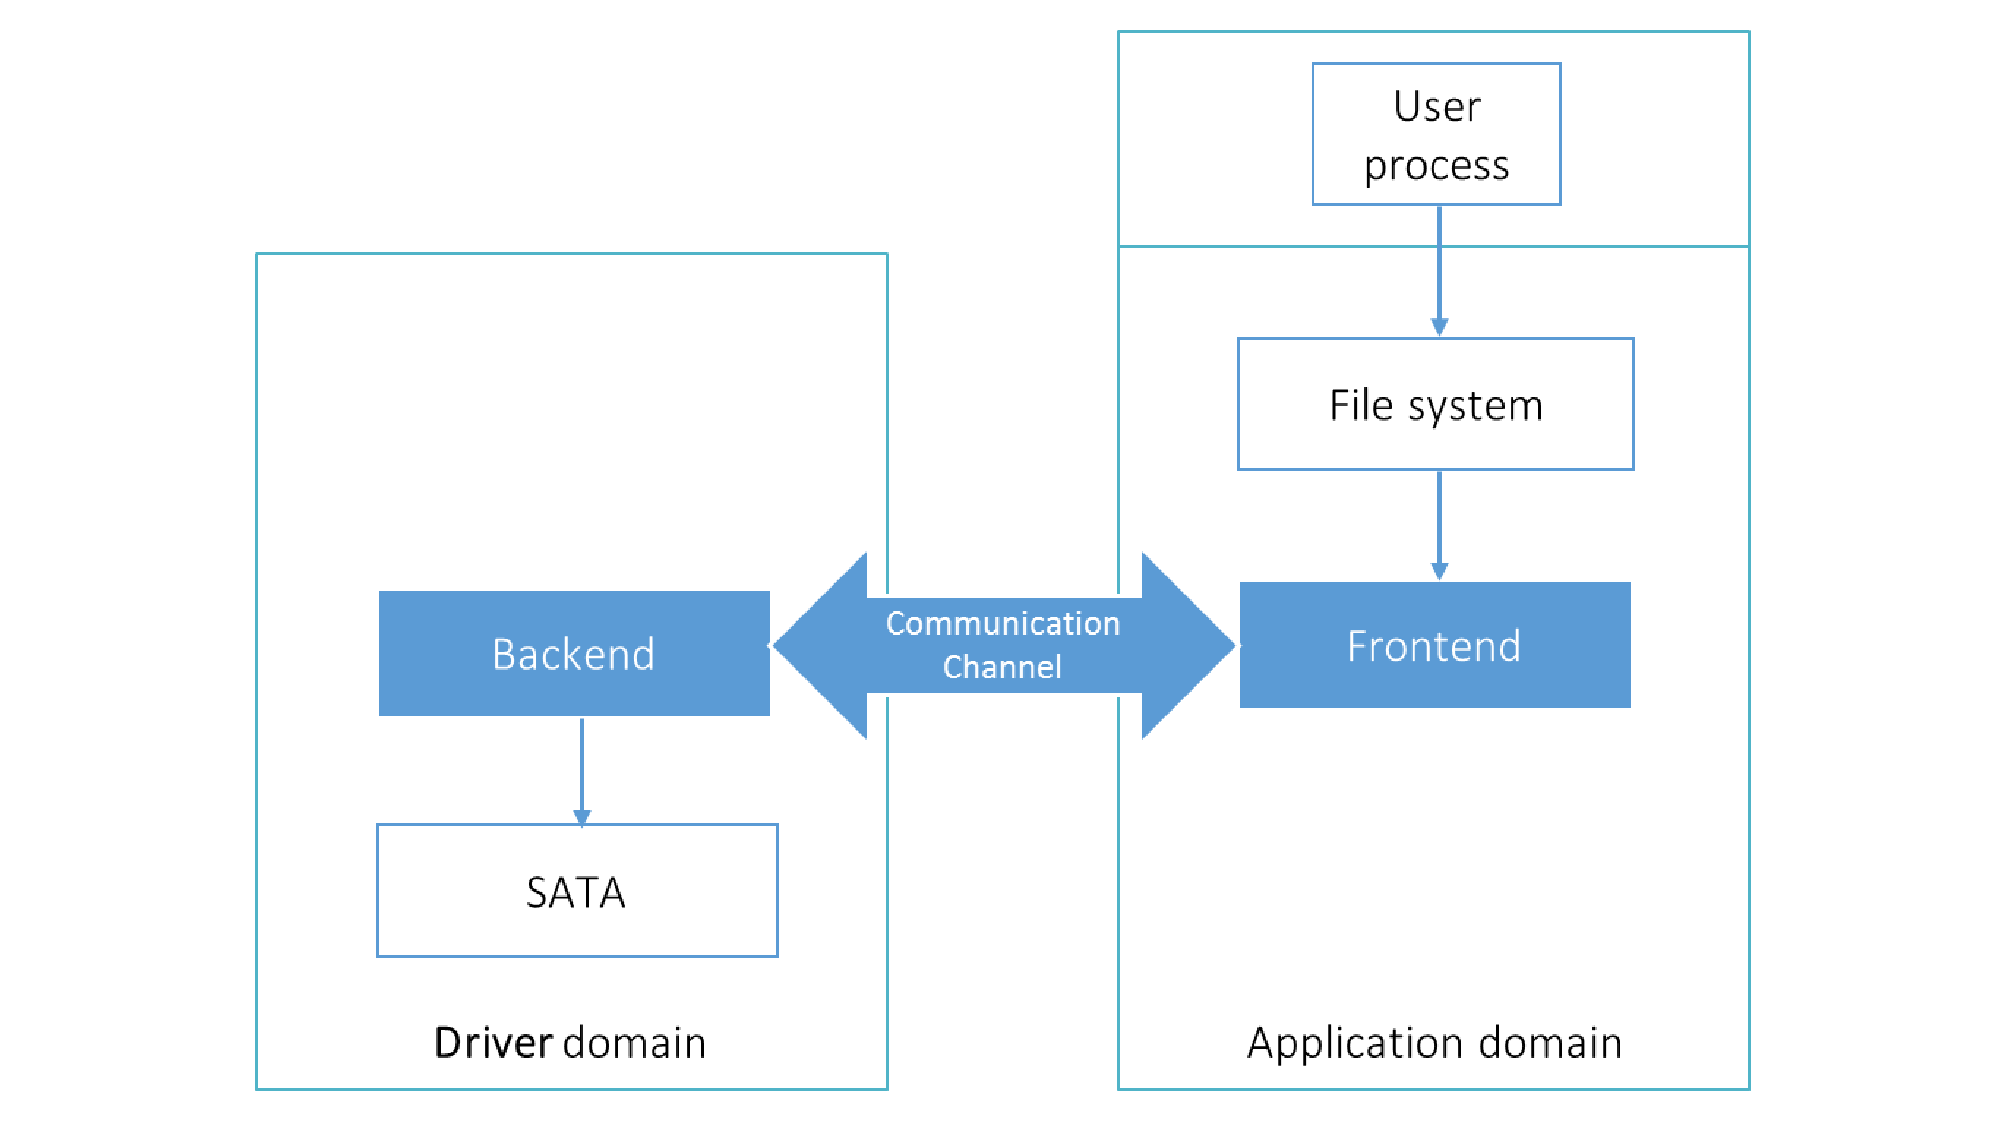
\includegraphics[scale=.5]{IDDRcomponents}
\caption{System Components}
\label{fig:Design Evo1}
\end{figure}

\subsection{Frontend Driver}
\label{subsec:frontend}

The IDDR system runs the \textit{frontend
driver} in the application domain. The \textit{frontend driver} acts
as a substitute or proxy for the actual device driver. The main purpose of the
\textit{frontend driver} is to accept requests from user applications,
process the requests, enqueue the requests for the driver domain and
notify the driver domain. The \textit{frontend driver} reads and processes
the responses received from the driver domain and notifies the caller
when the corresponding requests have been completed.  This notification
is referred to in the Linux kernel as ``ending the request''.

Without the frontend device driver, we would have had to change
existing applications in order to send requests to the actual device
driver running in the driver domain. Hence, the
frontend driver helps us achieve our transparency goal.

In the IDDR system, the frontend driver provides an interface to accept
requests from a user application on behalf of the device driver. 
As explained in Section~\ref{subsec:request queue}, each block device
driver has a separate request queue to accept requests from user
applications. Like all block device drivers, the frontend driver
creates an individual request queue for a device to accept requests.
The frontend driver submits the requests to the
communication channel. The frontend driver receives a software interrupt
upon the availability of responses in the shared queue. The frontend
driver handles the software interrupt by reading data from the shared
memory in case of read operations and sends a completion notification to
a user application.  In the case of write operations, it only sends the
completion notification.

\begin{figure}[!ht]
\centering
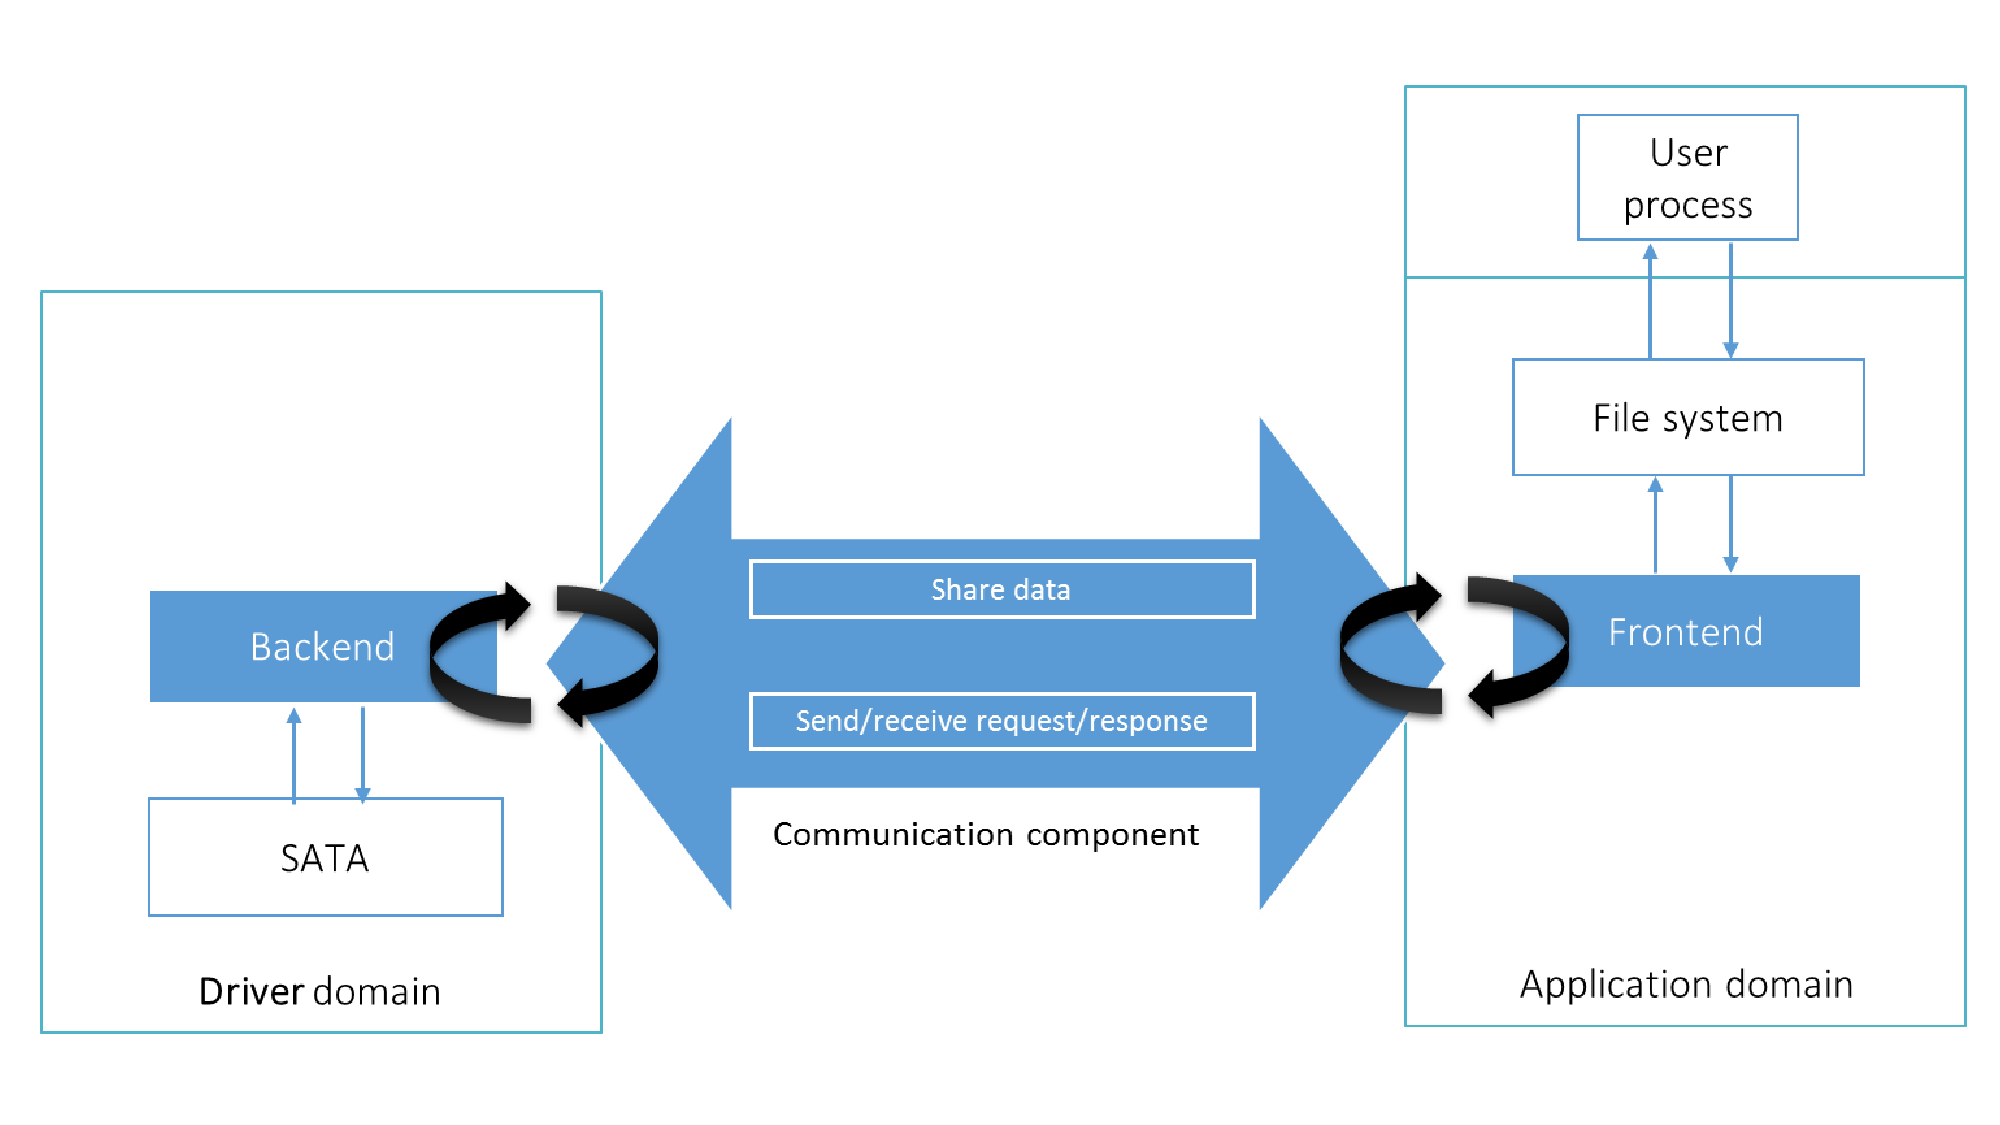
\includegraphics[scale=.5]{IDDRdesign}
\caption{Spinning based IDDR system}
\label{fig:new IDDR system}
\end{figure}
\subsection{Backend Driver}
\label{subsec:backend}
The IDDR system runs a \textit{backend driver}
runs in the driver domain. The responsibility of the \textit{backend
driver} is to accept requests from the application domain and forward
them to the actual device driver. The \textit{backend driver} sends
the responses and notifies the application domain after receiving the
responses from the device driver.

Without the backend device driver, we would have had to change existing device
drivers in order to send responses to user applications running in the
application domain. Hence, with introduction of the backend driver we
achieve the compatibility goal.

\begin{figure}[!ht]
    \centering
    \begin{subfigure}[b]{0.45\textwidth}
	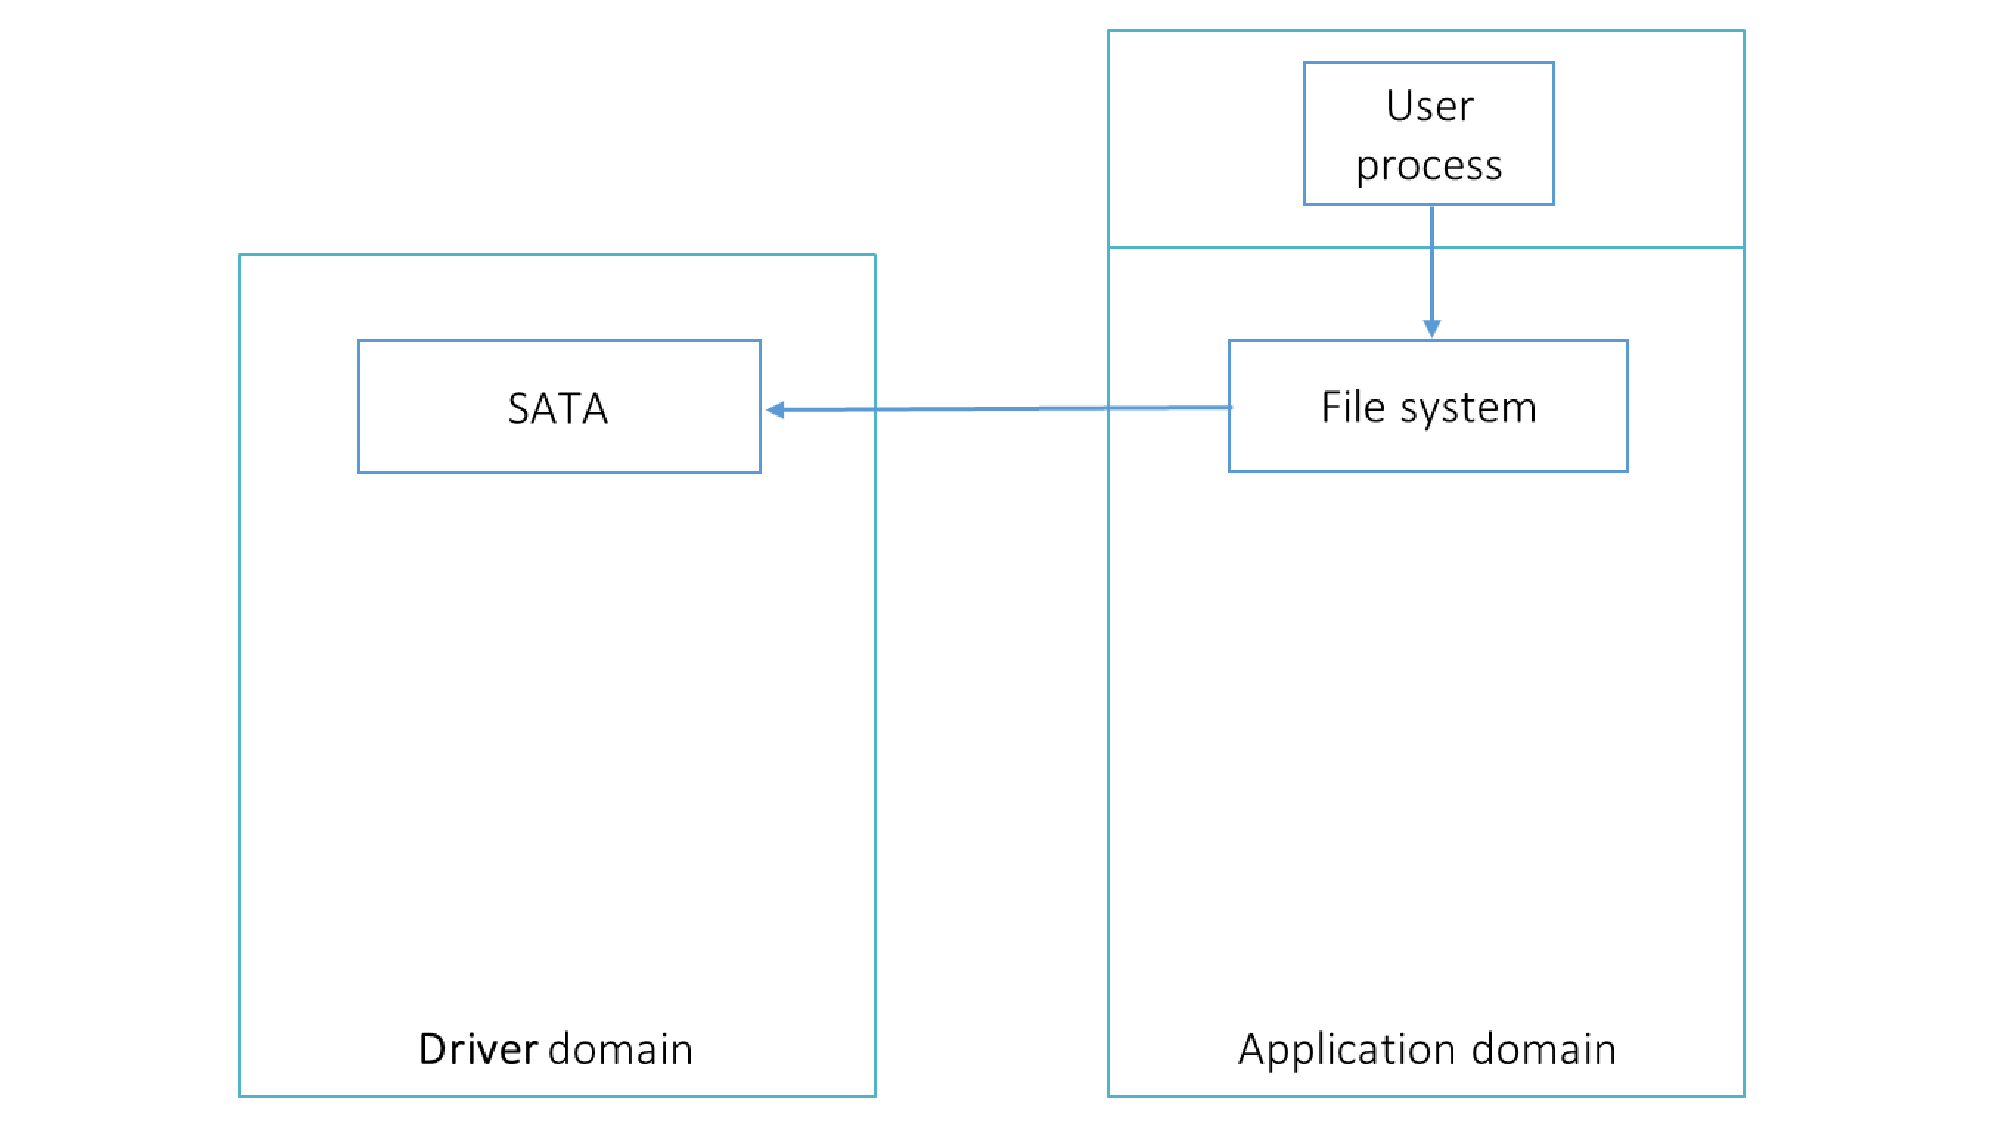
\includegraphics[scale=.25]{component1}
	\caption{Conceptual design of the driver domain}
	\label{fig:conept}
    \end{subfigure}
	\hfill
    \begin{subfigure}[b]{0.45\textwidth}
	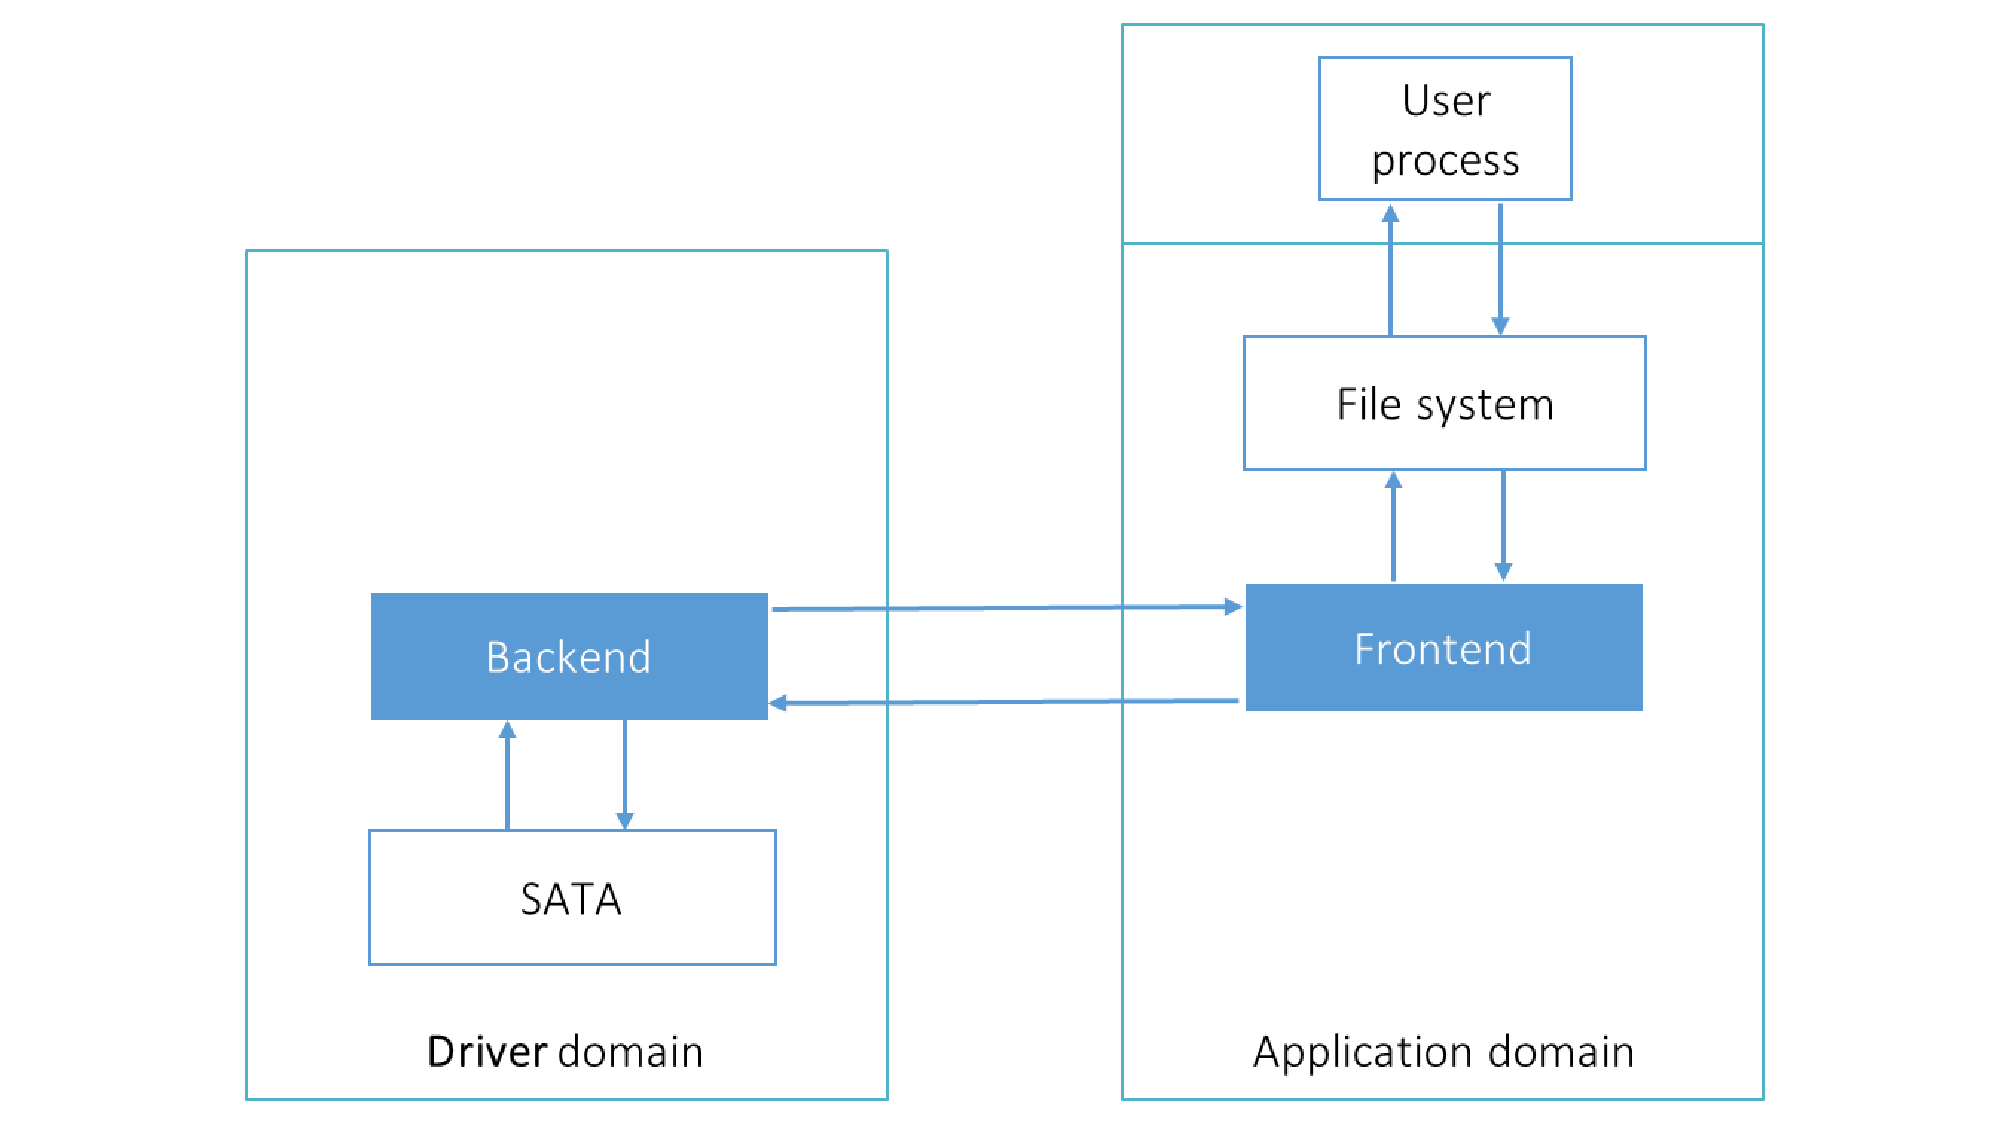
\includegraphics[scale=.25]{component2}
	\caption{Backend and frontend driver}
	\label{fig:backendfrontend}
    \end{subfigure}
    \caption{Role of the frontend and the backend drivers}\label{fig:fault tolerence}
\end{figure}

\subsection{Communication Module}
\label{sub:communicationmodule}

The communication module provides a communication channel between
the \textit{frontend driver} and the \textit{backend driver}. The
communication channel is logically divided into three parts. The
responsibility of the communication module is to

\begin{enumerate} 
\item share the requests and responses between the driver domain and the application domain.
\item manage and share the data of read/write requests/responses.
\item notify the domain upon the occurrence of events such as when requests or responses are produced. 
\end{enumerate}

Figure~\ref{fig:communication} provides an overview of the communication module. 
\begin{figure}[!ht]
\centering
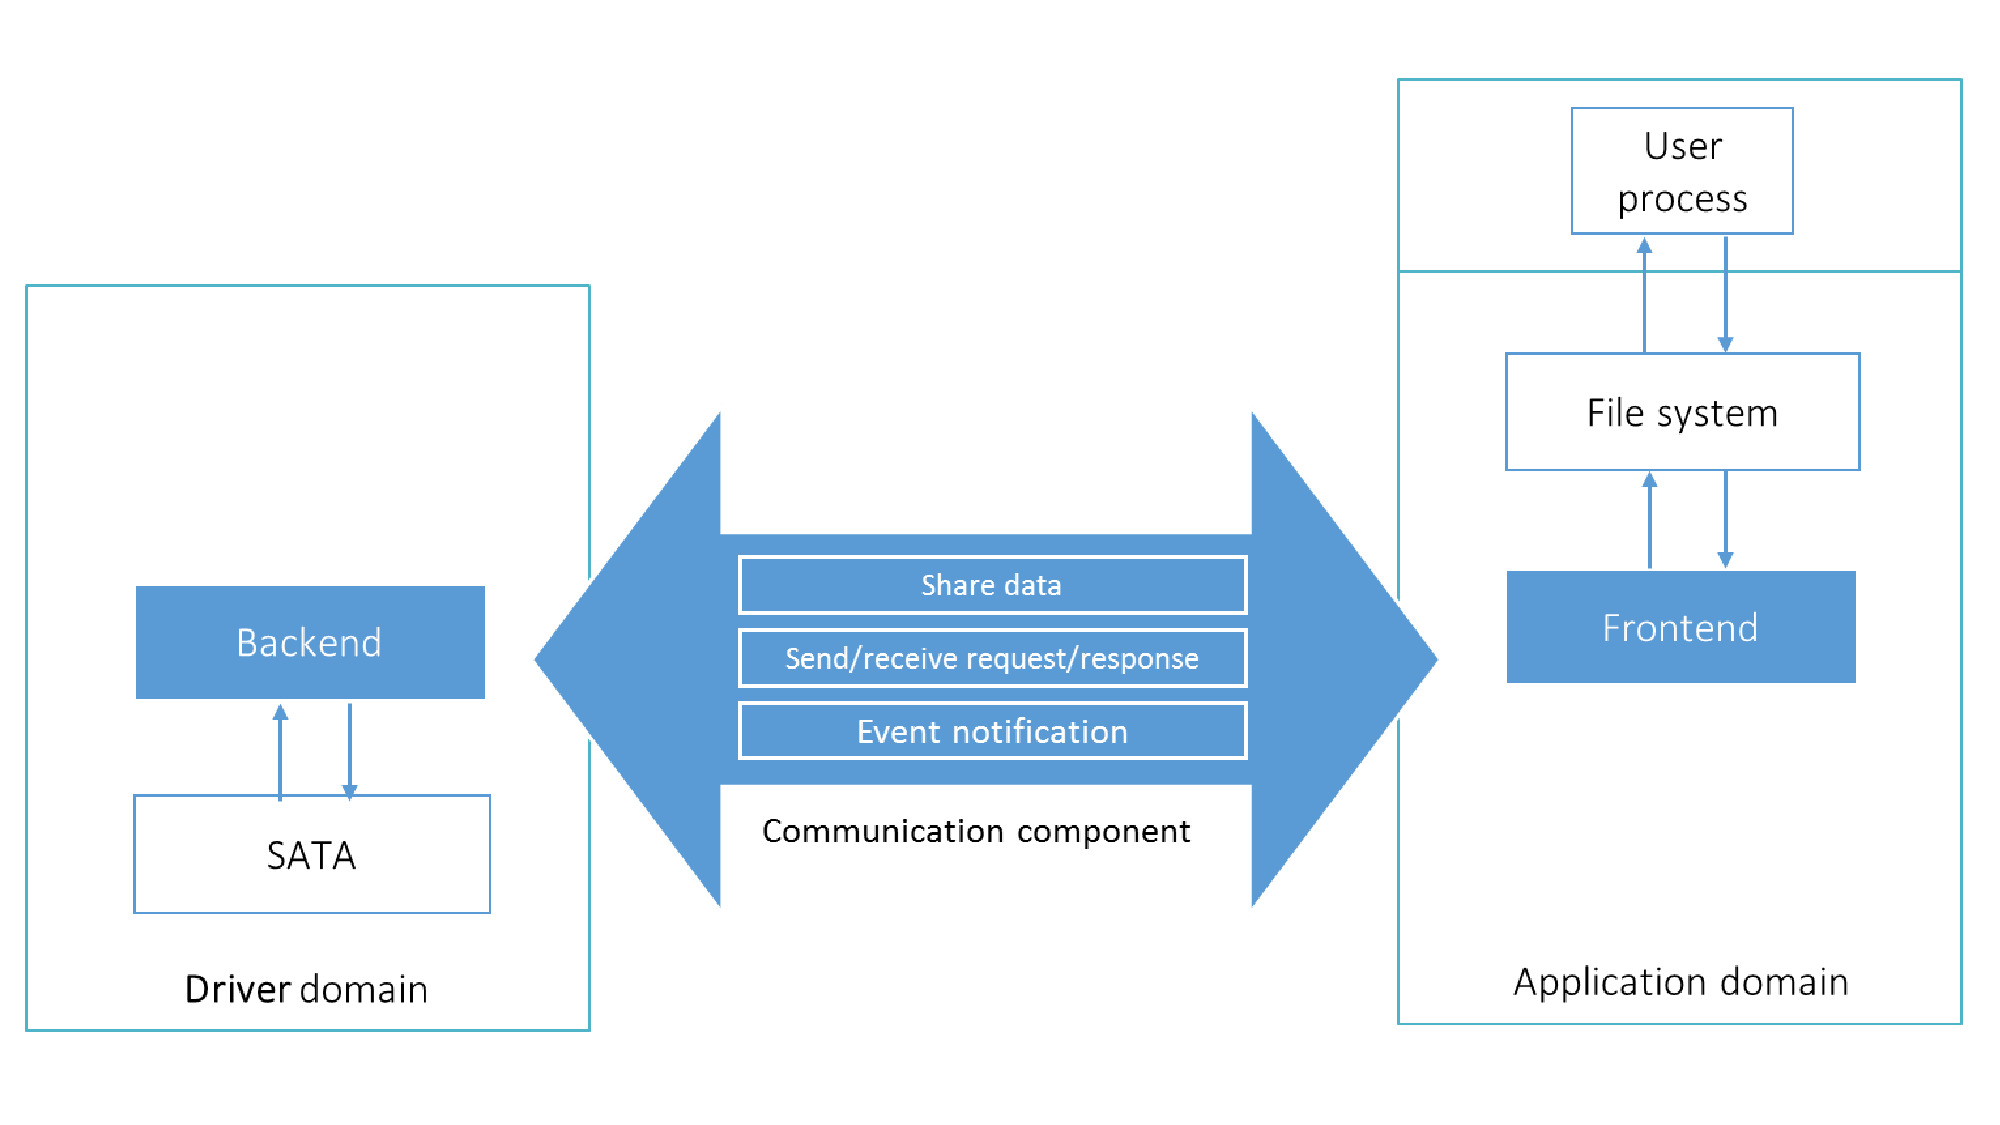
\includegraphics[scale=.5]{communicationmodule}
\caption{Communication Module}
\label{fig:communication}
\end{figure}

\paragraph{Interrupt based IDDR System:}
\label{par:base IDDR communication}
In the interrupt based approach, the frontend driver submits requests
to the communication module. The communication module copies the data of
the write requests to shared memory. The communication module is
responsible for the allocation and de-allocation of the shared memory
pages. Once a sufficient number of requests is submitted by the frontend
driver, the communication channel shares the requests with the backend
driver. It notifies the backend driver that requests are available in
the shared request queue.

\paragraph{Spinning based IDDR System:}
\label{par:spin IDDR communication} In the interrupt based approach, by
default a software interrupt is sent to the domain as a notification. Each
such software interrupt causes the hypervisor to schedule the driver
domain. Similarly, software interrupts which notify the availability of
responses, causes the hypervisor to schedule the application domain. The
scheduling of the driver domain and the application domain might result
in a context switch.

In order to avoid these context switches, we run an intermediate
thread in the frontend driver and an intermediate thread in the backend
driver. Both threads spin for the availability of requests and responses
in the shared queue. The intermediate threads delegate the responsibility
of the notifications from the frontend driver and backend driver to the
communication module.
